\section{Redis}

Redis merupakan basis data sumber terbuka berbasiskan \textit{key-value store}. Redis mendukung berbagai tipe data, mulai dari string, bitmap, bitfield, hash, list, set, dan lain-lain. Selain itu, Redis merupakan basis data yang menyimpan data pada memori dan berjalan secara \textit{single thread} sehingga Redis berjalan dengan cepat dan tidak perlu menangani konkurensi. Selain itu, Redis memiliki banyak dukungan fitur seperti dukungan persistensi dengan \textit{snapshot} atau \textit{append-only file} (AOF), dukungan \textit{high-availability}, replikasi, pemartisian, \textit{publisher-subscriber}, \textit{stream}, dan lain-lain \parencite{redisExplained}.

Konfigurasi Redis Cluster memungkinkan penskalaan secara horizontal dengan menyebarkan data pada mesin. Redis menggunakan fungsi hash deterministik untuk mendistribusikan data. Selain itu, Redis menggunakan \textit{gossip protocol} untuk menilai keadaan kluster. Ketika \textit{master} tidak responsif, node \textit{secondary} dapat dipromosikan menjadi node \textit{primary} \parencite{redisExplained}. Konsep umum lain pada Redis diilustrasikan pada gambar \ref{fig:redis-explained}.

\begin{figure}[htbp]
    \centering
    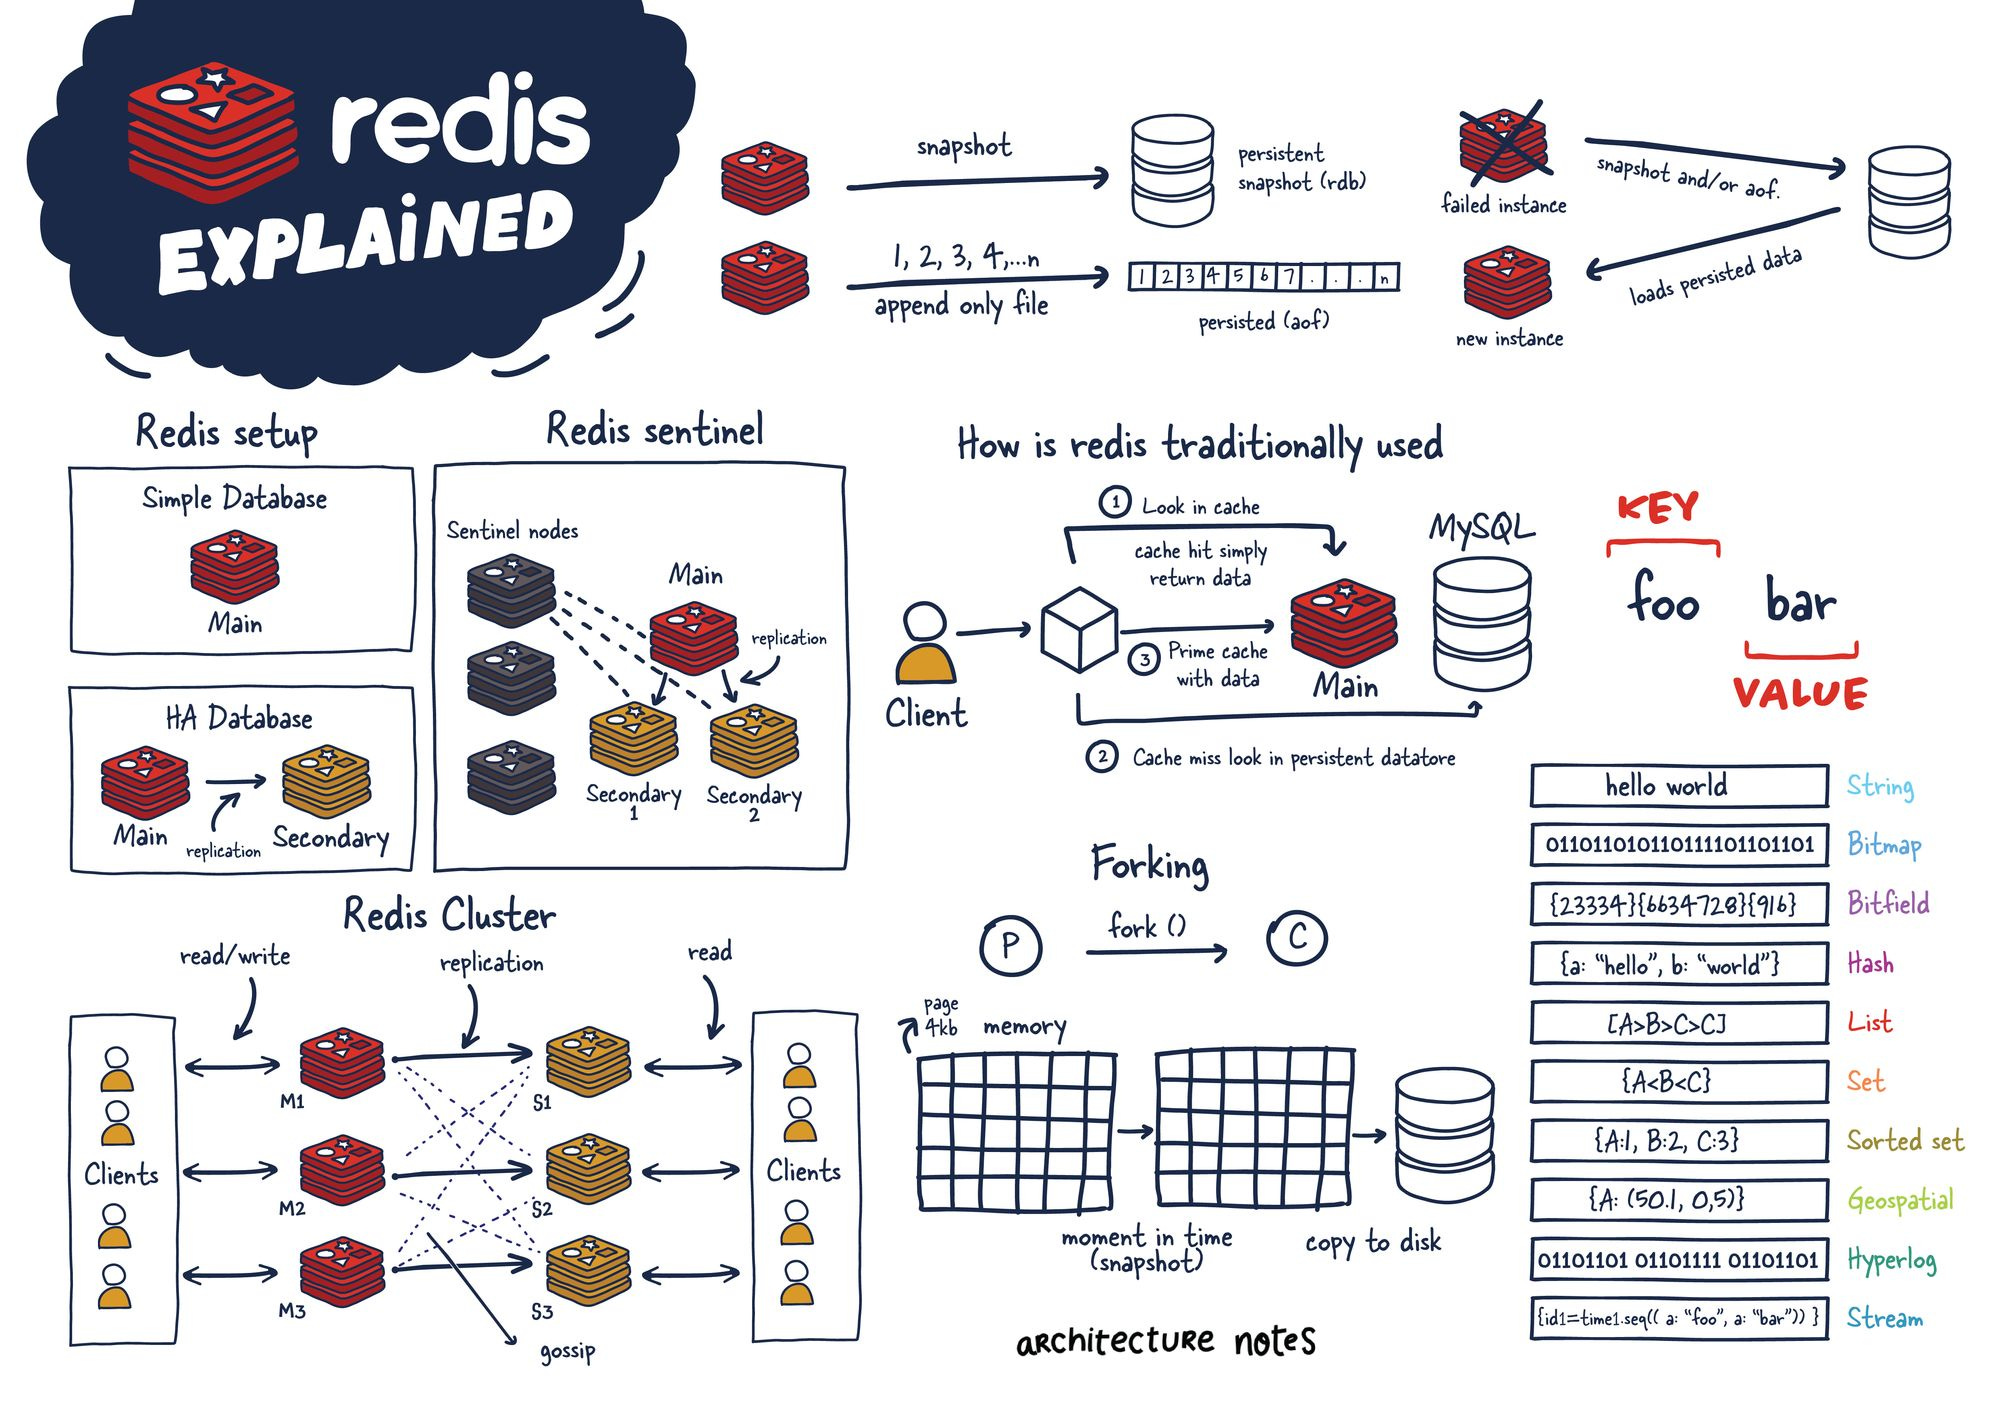
\includegraphics[width=1\textwidth]{resources/chapter-2/redis.jpg}
    \caption{\textit{Redis Explained \parencite{redisExplained}}}
    \label{fig:redis-explained}
\end{figure}
